\chapter{Methodology - Model Specification and Architecture}

\section{Instance-based Explainability Methods}
asdf
\fxnote{Establish setting of instance-based and furthermore gradient-based explanations, etc.}
\section{Gradient Similarity as a Method for Explanation}
asdf

\section{Fine-Tuning Setting}
Given a fine-tuning training dataset $D = \{s_i\}_{i=0}^N$, where $s_i$ is the $i$-th sample that contains a sequence of tokens. In the scope of this article, the term \emph{original} refers to samples in this dataset. Each of these samples contains instructions and generations, where $s_i^{-P_i},...,s_i^{-1}$ denote the tokens of the $i$-th instruction prompt of length $P_i$, and $s_i^0,...,s_i^{G_i}$ denote the tokens of the $i$-th generation for the $i$-th prompt with a length of $G_i$.
\\\\
Then the training of an \acrshort{llm} can be formulated as follows: 
\begin{equation}
    \hat{\theta} = \arg\min_{\theta} \frac{1}{\sum_{i=0}^{N} G_i} \sum_{i=0}^{N} \sum_{j=0}^{G_i} \mathcal{L}(s_i^j, \theta)
    \label{eq:llm_loss_function}
\end{equation}
where $\theta$ represents the parameters of the model and $\mathcal{L}(\cdot, \theta)$ is the loss function. The term $\frac{1}{\sum_{i=0}^{N} G_i}$ in equation \ref{eq:llm_loss_function} is the total number of generation tokens in the entire training set. Usually, for the \acrshort{llm} objective, the loss is $\mathcal{L}(s_i^j, \theta) = -\log p_\theta(s_i^j \mid s_i^{-P_i}, \ldots, s_i^{j-1})$ the negative log-likelihood of the correct token given all previous tokens. \fxnote{Maybe explain where the probabilities are coming from --> softmax} Modern \acrshort{llm} architectures use adapted versions of it or may use other loss functions. However, in this setting, the choice of loss function does not matter as long as it suits language modeling. Let $\mathcal{L}(s_i, \theta) = \frac{1}{G_i} \sum_{j=0}^{G_i} \mathcal{L}(s_i^j, \theta)$, be the loss per sample which will be relevant in the following sections.
\\\\
Usually, machine learning models are trained using batches of training data with size $b > 1$. In the setting of this article, the batch size is set to $b = 1$ to measure phenomena for single instances. Hence, in the training process, for iteration $a$, the parameters are updated from $\theta_{a-1}$ to $\theta_{a}$ depending on the training sample $s_a$. 
\\\\
Modern \acrshort{llm} training still relies on the original idea of gradient descent to update the model weights despite being more advanced in terms of convergence, regularization, memory-efficiency, etc., for example, LAMB \cite{you2020largebatchoptimizationdeep}. However, in the proposed setting, we are only looking at the gradients of the loss function with respect to each individual training sample without updating the model weights correspondingly; therefore, establishing the idea of gradient descent is sufficient here. The formulation of gradient descent for this setting is shown in equation \ref{eq:gradient_descent}:
\begin{equation}
    \theta_{a+1} = \theta_a - \eta_a \nabla_{\theta} \mathcal{L}(s_a, \theta_a)
    \label{eq:gradient_descent}
\end{equation}
where $\eta_a$ is the learning rate in iteration $a$ and $\nabla_{\theta} \mathcal{L}(s_a, \theta_a)$ denotes the gradient of the loss function given $s_a$ and the current model parameters $\theta_a$ with respect to $\theta$. \cite{lin2024tokenwiseinfluentialtrainingdata}. In other words, the gradients determine how the model weights are updated based on the given training data. Hence, the gradient $\nabla_{\theta} \mathcal{L}(s_a, \theta_a)$ contains information on how the model parameters $\theta$ will be updated depending on the training data sample $s_a$. With this in mind, the effect of the gradient based on single samples will be analyzed in detail in the following chapters.
\fxnote{should I cite gradient descent, etc.?}

\section{Paraphrasing a Dataset}
The idea is to take a dataset $D$ on which a model was fine-tuned and paraphrase it using another \acrshort{llm}. When paraphrasing, we obtain $D_p = \{s_{p_i}\}_{i=0}^N$, a dataset where the inputs and the outputs, in other words, the prompt and the generation, are paraphrased. Hence, the semantics of the samples are preserved, while the syntax and word choice differ between $D$ and $D_p$. For that, the prompt and the generation for each sample $s_i$ are individually paraphrased to retrieve a new sample $s_{p_i}$, as illustrated in Equation \ref{eq:paraphrasing}. As a reminder, each sample is basically a tuple containing an instruction and a generation. For simplicity, let us introduce $s_{i_P}$ and $s_{i_G}$ which represent the prompt and the generation of the $i$-th sample, respectively, such as $s_i = (s_{i_P}, s_{i_G}) = (s_i^{-P_i},...,s_i^{-1}, s_i^0,...,s_i^{G_i})$.
\begin{equation}
    s_{p_i} = 
    (
    s_{p_{i_P}},
    s_{p_{i_G}}
    ) =
    (
        s_{p_i}^{-P_i},...,s_{p_i}^{-1},
        s_i^0,...,s_{p_i}^{G_i}
    ) = 
    (
        \operatorname{LLM_{para}}(s_{i_P}), 
        \operatorname{LLM_{para}}(s_{i_G})
    )
    \label{eq:paraphrasing}
\end{equation}
As mentioned above, $s_{p_i}$ denotes the paraphrased version of the $i$-th sample representing a tuple of the paraphrased prompt $s_{p_{i_P}}$ and the paraphrased generation $s_{p_{i_G}}$. The function $LLM_{para}$ in Equation \ref{eq:paraphrasing} basically represents an \acrshort{llm} that is used to paraphrase a sequence of tokens as mentioned above and will be further illustrated in Section \ref{sec:paraphrasing_samples}.
\\\\
Furthermore, another paraphrasing setting is established by using the model under evaluation to generate the output with the paraphrased instruction prompt $s_{p_{i_P}}$ as input. This basically generates another dataset $D_m = \{s_{m_i}\}_{i=0}^N$ that is used for further evaluation in this context. As the other samples of the datasets $D$ and $D_p$, each sample $s_{m_i}$ of $D_m$ represents a tuple of prompt $s_{m_{i_P}}$ and generation $s_{m_{i_G}}$, as shown in Equation \ref{eq:model_generated_sample}.
\begin{equation}
    s_{m_i} = 
    (
    s_{m_{i_P}},
    s_{m_{i_G}}
    ) =
    (
        s_{p_i}^{-P_i},...,s_{p_i}^{-1},
        s_{m_i}^0,...,s_{m_i}^{G_i}
    ) = 
    (
        s_{p_{i_P}}, 
        \operatorname{LLM}(s_{p_{i_P}})
    )
    \label{eq:model_generated_sample}
\end{equation}
Technically, $s_{m_{i_G}} = s_{p_{i_G}}$, but for clarity $s_{m_{i_G}}$ will be denoted independently to establish its affiliation to $D_m$ and not be confused with an instruction for a sample in $D_p$. The function $LLM(\cdot)$ in Equation \ref{eq:model_generated_sample} basically returns the generation of the current \acrshort{llm} under evaluation and takes in a sequence of tokens $s_i^{-P_i},...,s_i^{-1}$. The dataset $D_m$ is generated to add an additional layer of obfuscation when considering the original $D$ and the paraphrased one $D_p$.
\\\\
Given that, the following two settings are established and, for simplicity, will be named accordingly in the following article:
\begin{itemize}
    \item \textbf{Paraphrased}: This setting refers to the evaluations regarding the dataset $D_p$. Samples $\spi$ in this setting will be called paraphrased samples.
    \item \textbf{Model-Generated}: This setting refers to the evaluation regarding the dataset $D_m$. Alternatively, in this setting, the samples $\smi$ will be called model-generated samples.
\end{itemize}

\section{Language Model Components}
Modern \acrlong{llm}s still rely on the Transformer architecture to create appropriate text based on an input prompt. In other words, autoregressive language models, for example, the \acrfull{gpt} model series from OpenAI, predict tokens based on a sequence of input tokens using an adapted decoder-only architecture inspired by the original Transformer \cite{vaswani2023attentionneed}.

\subsection{Different Layers and Components}\label{ssec:different_layers_and_components}
Hence, we have many trainable parameters from different components. Some of them, for example, activation functions, input layer normalization, post-attention layer normalization, etc., usually included in every \acrlong{llm}, are not trainable and therefore no gradient of the loss function with respect to these components is calculated. For a generic \acrshort{llm} that takes in a sequence of tokens, we might have the following trainable parameters without considering positional encoding, etc.:
\begin{itemize}
    \item \textbf{Input Embedding}: This parameter takes in an already tokenized and encoded sequence and transforms it into the embedding space using, for example, a matrix $\mathbf{E} \in \mathbb{R}^{|V| \times d_x}$. 
    
    \item \textbf{Multiple Transformer Block}:
    Each transformer block is applied multiple times depending on the model architecture. A generic transformer decoder consists of:
    \begin{itemize}
        \item \textbf{Self-Attention}: Three matrices representing the query, key, and value weights in self-attention:
            \begin{align*}
                  \mathbf{W}^{(q)} \in \mathbb{R}^{d_x \times d_q},  
                  \mathbf{W}^{(k)} \in \mathbb{R}^{d_x \times d_k},  
                  \mathbf{W}^{(v)} \in \mathbb{R}^{d_x \times d_v}.
            \end{align*}\cite{dl4nlp}
        \item \textbf{Multiple MLP Projections}: Each transformer block also contains a position-wise feed-forward network (in this example, a two-layer MLP). For every block, the model learns
            \begin{align*}
              \mathbf{W}^{(1)} &\in \mathbb{R}^{d_x \times d_{ff}}, & \mathbf{b}^{(1)} &\in \mathbb{R}^{d_{ff}},\\
              \mathbf{W}^{(2)} &\in \mathbb{R}^{d_{ff} \times d_x}, & \mathbf{b}^{(2)} &\in \mathbb{R}^{d_x},
            \end{align*}
              where $d_{ff}$ is the hidden width of the MLP. It can be written as one liner: $\text{MLP}(x)=\mathbf{W}^{(2)}\!\bigl(\text{ReLU}(\mathbf{W}^{(1)}x+\mathbf{b}^{(1)})\bigr)+\mathbf{b}^{(2)}$, where $x$ is a training sample or in the case of \acrlong{llm}s, the output of a previous layer component.
    \end{itemize}
    
    \item \textbf{Output Embedding}: A final linear layer projects the network output back to vocabulary logits. In some \acrshort{llm}s, the weights are tied to the input embedding \cite{press2017usingoutputembeddingimprove}:
          \begin{align*}
              \mathbf{W}^{(o)}=\mathbf{E}^{\!\top}\in\mathbb{R}^{d_x \times |V|}
          \end{align*}
          where $|V|$ is the size of the vocabulary. (Some models keep an independent $\mathbf{W}^{(o)}$ instead.)
\end{itemize}
As already mentioned, this is just a simplified illustration of the trainable parameters an \acrshort{llm} could have. In practice, the attention mechanism can be divided into multiple attention heads to capture different semantics in each head. For a detailed illustration of the Transformer decoder, see the original paper "Attention Is All You Need"~\cite{vaswani2023attentionneed}. Now that the notion of some trainable parameters for \acrlong{llm}s is put into context, the original assumption of gradient similarity is established in the following sections.

\section{Gradient Similarity between Samples}
TODO: illustrate the general idea; use general notation of similarity between gradients of different samples.

\fxnote{the upcoming section only covers equation with $\spi$. make clear, that the calculation also are valid for $\smi$}

\subsection{Gradient Flattening}
Equation~\ref{eq:gradient_descent} illustrates how gradient descent updates the model parameters for training iteration $a$ and the current model parameters $\theta_a$. However, the setting in this article focuses on already fine-tuned models, and hence only the final model parameters $\theta_T$ are used for gradient computations. For example, the loss function gradient for a sample $s_i$ and the trained model parameters $\theta_T$ w.r.t. the model parameters $\theta$ is denoted as $\nabla_{\theta} \mathcal{L}(s_i, \theta_T)$.
\\\\
As illustrated in Subsection~\ref{ssec:different_layers_and_components}, the model parameter space $\theta$ consists of many different variations of matrices with different sizes and dimensions. For simplicity, denote the parameter space $\theta$ as a generic set of parameter matrices
$\{\Wlk\}_{l=0}^L$, where $\Wlk \in \RnWlkXdWlk$. Here, $L$ denotes the number of layers, and $k$ just the $k$-th weight in layer $l$, where $k \in 0,\dots,K_l$ and $K_l$ is the number of weights inside layer $l$. Depending on which \acrshort{llm} is used, the number of layers $L$, the weights inside these layers, and the dimensions of those weights $\RnWlkXdWlk$ differ in size and dimension. The size of the model, in other words, the number of trainable parameters a model has, is shown in Equation \ref{eq:number_model_parameters}.
\begin{equation}
    M = \sum_{l=0}^{L} \sum_{k=0}^{K_l} \nWlk + \dWlk
    \label{eq:number_model_parameters}
\end{equation}
As an example, today, there are many different \acrlong{llm}s with different sizes, for example, Llama 3.1 consists of 405 billion parameters \cite{grattafiori2024llama3herdmodels} and, hence, for Llama 3.1, $M \approx 405,000,000,000$.
\\\\
For simplicity, call $\nabla_{\theta} \mathcal{L}(s_i, \theta_T)$ the full model gradient for sample $s_i$. To compute this full model gradient, the gradients w.r.t. to each model weight $\nabla_{\mathbf{W}^{(l,k)}} \mathcal{L}(s_i, \theta_T) \in \RnWlkXdWlk$ have to be calculated and combined to represent the gradient w.r.t. the whole parameter space. After the computation of each individual weight gradient $\nabla_{\Wlk} \mathcal{L}(s_i, \theta_T)$, they are flattened into a gradient vector that can be calculated as: 
\begin{align*}
    \mathbf{v}_{\Wlk}(s_i)
    \;:=\;
    \operatorname{vec}_r\!\bigl(\nabla_{\Wlk}\mathcal L(s_i,\theta_T)\bigr)
    \;\in\;\mathbb R^{\,\nWlk\dWlk}.
\end{align*}
The row-major vectorization function $\operatorname{vec}_r(\cdot)$, is the mapping $\operatorname{vec}_r:\mathbb{R}^{m \times n} \to \mathbb{R}^{mn}, \quad \mathbf{a} = \operatorname{vec_r}(\mathbf{A})$, where $\mathbf{A} = [A_{ij}] \in \mathbb{R}^{m \times n}, \quad i = 0, \ldots, m-1, \quad j = 0, \ldots, n-1$. Then this row-major vectorization is explicitly written as follows:
\begin{align*}
    \mathbf{a} = \operatorname{vec}_r(\mathbf A)=
    \begin{bmatrix}
    A_{0,0}\\ A_{0,1}\\ \cdots\\ A_{0,n-1}\\
    A_{1,0}\\ A_{1,1}\\ \cdots\\ A_{1,n-1}\\
    \vdots\\
    A_{m-1,0}\\ \cdots\\ A_{m-1,n-1}
    \end{bmatrix}
    \;\in\;\mathbb{R}^{mn}.
\end{align*}
\cite{curtarelli2023generalizedvectorizationinverse}. For example,
\begin{align*}
    \mathbf A=
    \begin{bmatrix}
    1 & 2 & 3\\
    4 & 5 & 6
    \end{bmatrix} \;\in\; \mathbb{R}^{2\times3}, 
    \quad 
    \operatorname{vec}_r(\mathbf A)=
    \begin{bmatrix}
    1\\2\\3\\4\\5\\6
    \end{bmatrix}.
\end{align*}
To combine all vectorized layer gradients $\mathbf{v}_{\Wlk}(s_i)$ for sample $s_i$, define the collector operator $\operatorname{col(\cdot)}$ as follows:
\begin{align*}
    \operatorname{col}(x_1,\dots,x_m) \;:=\;
    \begin{bmatrix}
    x_1 \\ \vdots \\ x_m
    \end{bmatrix} \; \in \; \mathbb{R}^{\sum_{j}{d_j}}, \quad \text{where} \; x_j \in \mathbb{R}^{d_j}.
\end{align*}
With the above properties and operators in mind, the full flattened gradient vector for sample $s_i$ is defined as 
\begin{align*}
    \vXsi[\theta]
\;:=\;
\operatorname{col}\bigl( \vXsi[\W^{(0,0)}], \vXsi[\W^{(0,1)}], \dots, \vXsi[\W^{(L,K_L)}] \bigr)
\; 
\in\; \mathbb{R}^{M}.
\end{align*}
For better understanding, the whole gradient flattening process covered in this subsection is illustrated in Figure \ref{fig:gradient_flattening}.
\begin{figure}[ht]
    \centering
    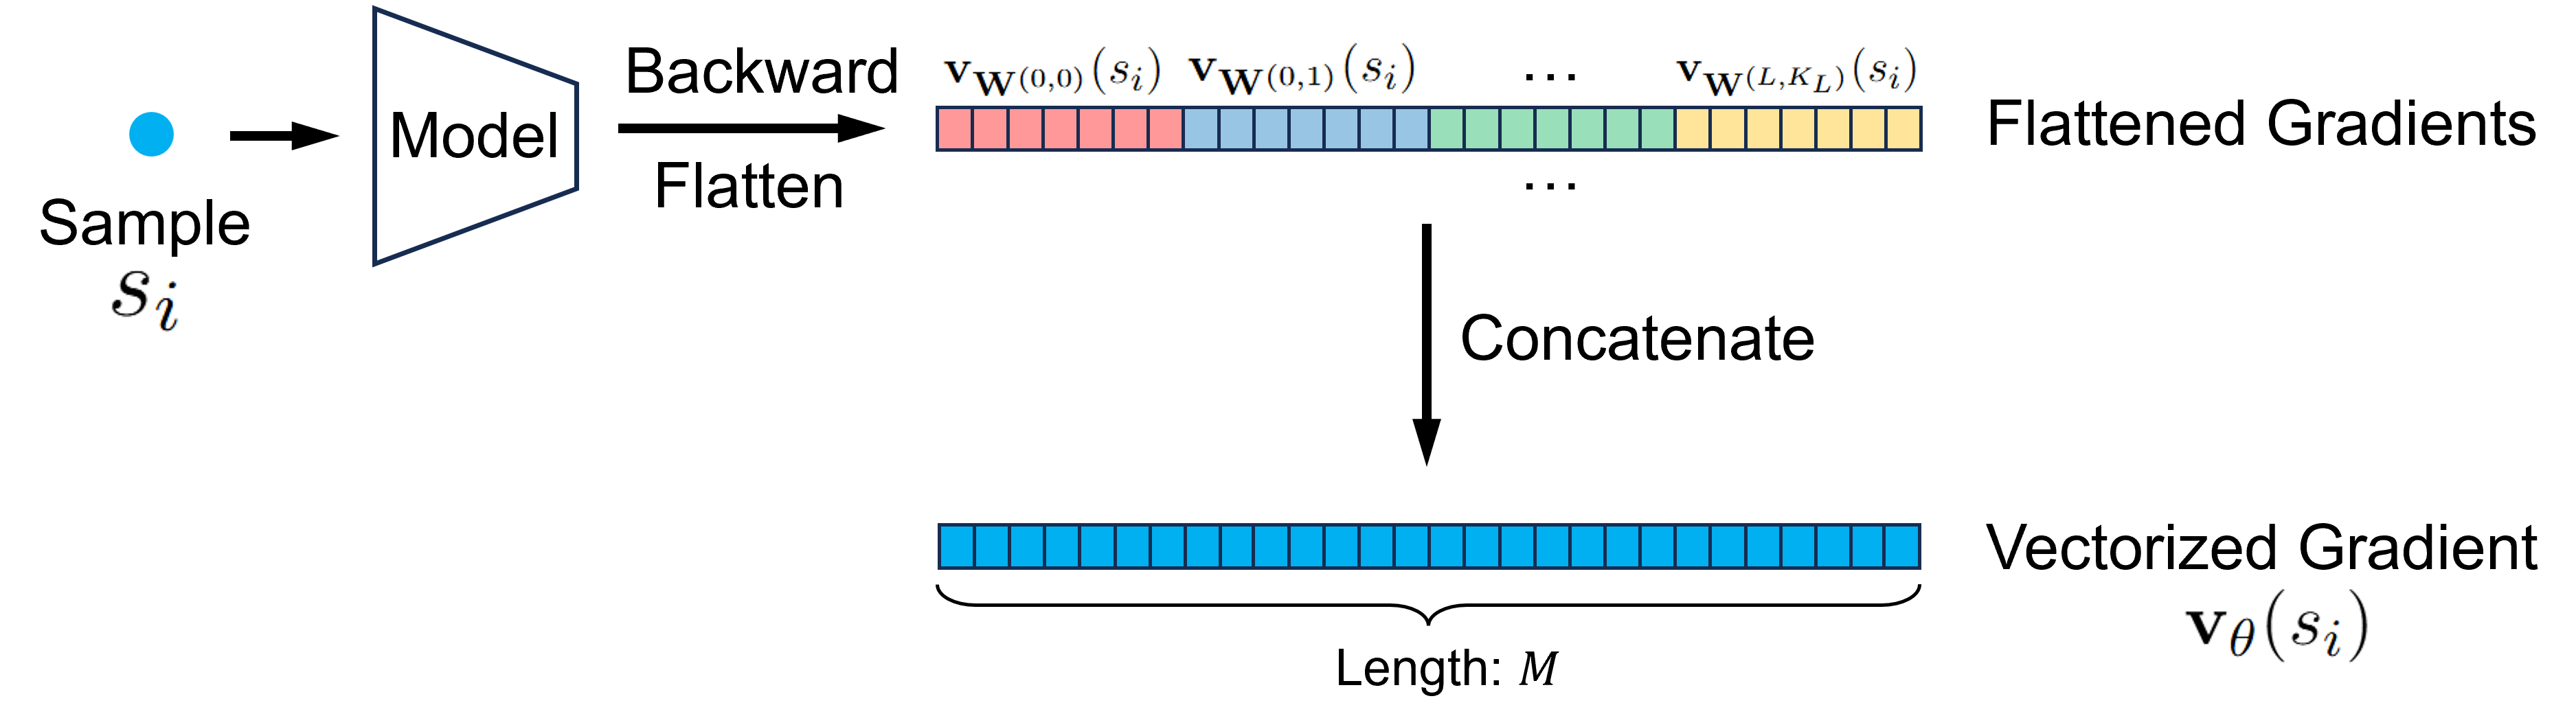
\includegraphics[width=1\textwidth]{figures/gradient_flattening.png}
    \caption{Visual representation of gradient flattening for sample $s_i$.}
    \label{fig:gradient_flattening}
\end{figure}
As a result of the gradient flattening process and the notion of $\vXsi[\theta]$, these vectorized representations of the gradients for different samples can be compared. In other words, the similarity between these can be calculated, which is elaborated in the following section.

\subsection{Similarity Measure}
Generally, a similarity measure is a real-valued function that quantifies the
similarity between two entities.  There are many different ways to measure the
similarity between two mathematical objects such as vectors.  Norms can be used
to measure the distance between two points in space, for example, the $L_1$-
and the $L_2$-norm, called the Manhattan and Euclidean norms, respectively.
Another way of measuring the similarity between two vectors is the dot product.

\subsubsection{Magnitude versus Direction}
The standard dot product between two non-zero vectors
$\mathbf{a},\mathbf{b}\in\mathbb{R}^d$ is defined as
\begin{align*}
    \mathbf{a}^{\top}\mathbf{b}
    \;=\;
    \|\mathbf{a}\|\,\|\mathbf{b}\|\cos{\varphi},
\end{align*}
where $\varphi$ denotes the angle between them. Consequently, a large dot product can arise in two distinct ways:
\begin{enumerate}
    \item \textbf{Directional alignment}: If $\varphi$ is small (for example, $\cos{\varphi} \approx 1$), the vectors point in nearly the same direction and therefore encode similar information.
    \item \textbf{Magnitude imbalance}: Even when $\varphi$ is close to $90^{\circ}$ (poor alignment), the product can still be large if either $\|\mathbf{a}\|$ or $\|\mathbf{b}\|$ is large.
\end{enumerate}
The magnitude of computed gradients from a training set can vary greatly~\cite{sui2021representer} and sometimes blurs the real influence of the gradients in a training set when comparing their local influence on each other~\cite{barshan2020relatifidentifyingexplanatorytraining}. To isolate direction alone, one typically uses cosine similarity,
\begin{align*}
    \simcos(\mathbf{a},\mathbf{b})
    \;=\;
    \frac{\mathbf{a}^{\top}\mathbf{b}}
         {\|\mathbf{a}\|\,\|\mathbf{b}\|},
\end{align*}
which normalizes both vectors and depends solely on the angle~$\varphi$.

\subsubsection{Implications for gradient-based influence analysis}
Using cosine similarity for gradient comparison has three practical advantages:
\begin{enumerate}
    \item \textbf{Magnitude-invariance}: Two gradients affect the score only through their angle and not by their magnitude.
    \item \textbf{Sensitivity to local influence}: By basically ignoring large norm outliers, cosine similarity prioritizes gradients whose direction truly matches that of the comparing gradient, which is the criterion for local influence~\cite{barshan2020relatifidentifyingexplanatorytraining}.
    \item \textbf{Interpretability}: A score of $+1$ means perfect alignment, $0$ orthogonality, and $-1$ opposition, which provides an intuitive quantity of how similar the gradients are.
\end{enumerate}
In short, cosine similarity isolates geometrically relevant information (direction) while
ignoring the interference factor (magnitude), making it an appropriate choice for
gradient-based influence analysis~\cite{Hammoudeh_2024}.

\section{Gradient Similarity}
As already mentioned, the original assumption is that when a model is already trained on sample $\si$, then in the paraphrased setting
\begin{equation}
    \simcos \bigl( \vXspi, \vXsi \bigr) > \simcos \bigl( \vXspi, \vXsj \bigr), \qquad \forall\,j\in\{0,\dots,N\}\setminus\{i\}.
    \label{eq:cosine_similarity_paraphrased}
\end{equation}
That means that the full model gradient of the paraphrased sample $\spi$ is most similar to its original sample $\si$ compared to all other original samples $\sj$. If this is the case, then the gradient-based explanation method is able to find the original data point for its paraphrased equivalent. 
\begin{figure}[ht]
    \centering
    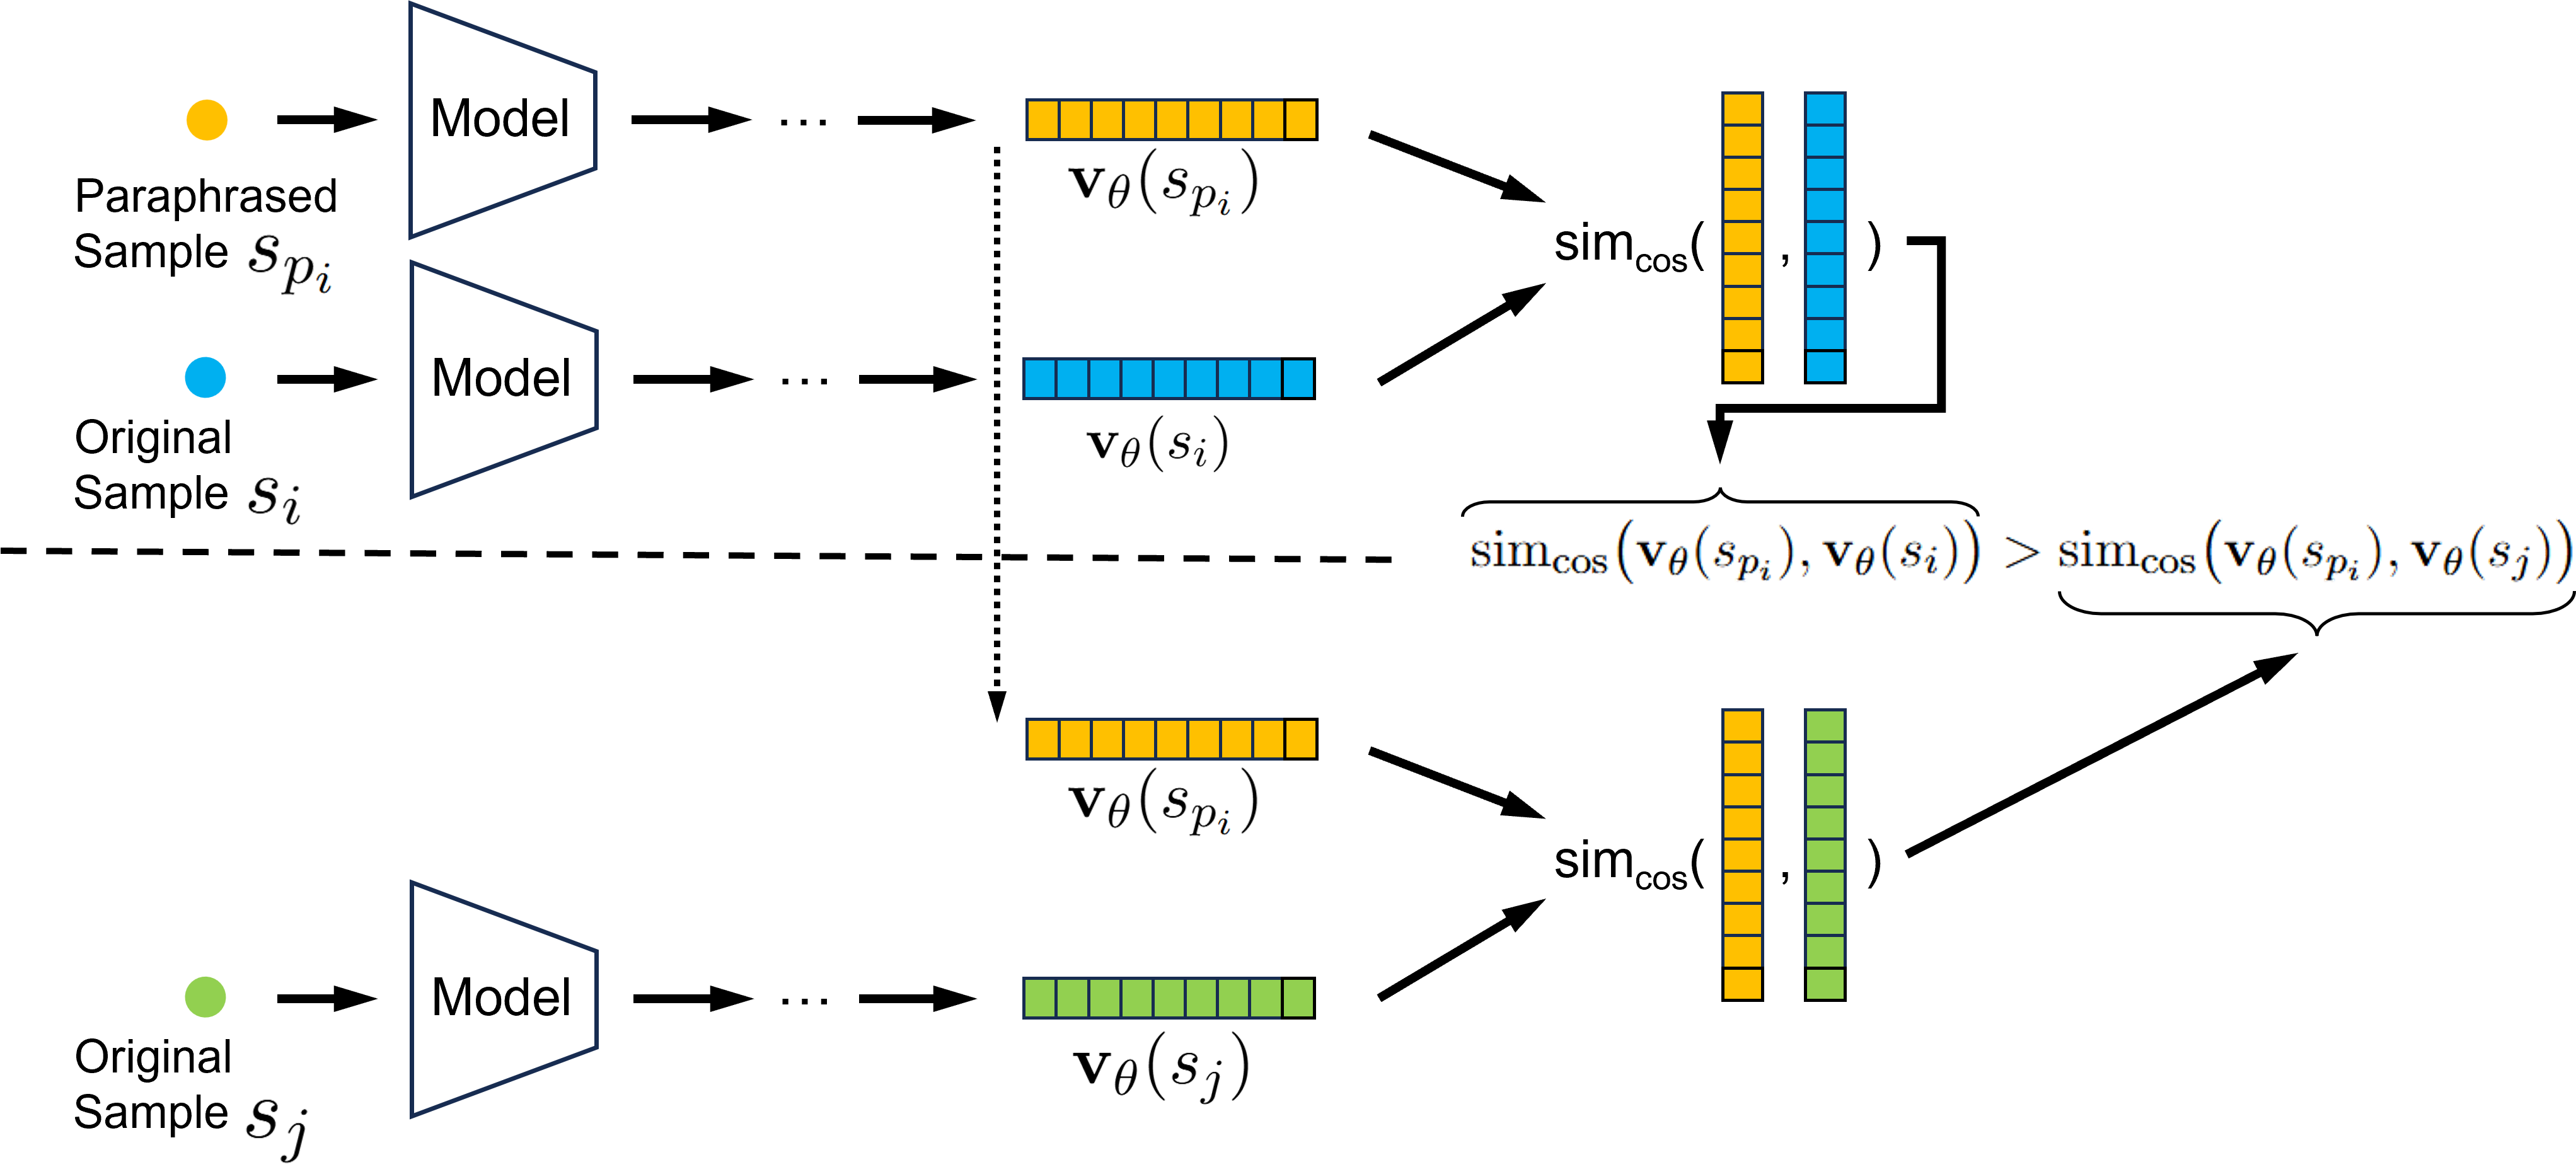
\includegraphics[width=1\textwidth]{figures/gradient_cosine_similarity.png}
    \caption{Visual representation of the gradient cosine similarity comparison between $(\spi, \si)$ and $(\spi, \sj)$.}
    \label{fig:gradient_cosine_similarity}
\end{figure}
For both settings, this comparison is made for all samples $\spi$ and $\smi$ to calculate a score of how well the model gradients can find the equivalent original data points. 
\begin{equation}
\operatorname{accuracy}_\theta(D_p, D)
\;:=\;
\frac{1}{N}\sum_{i=0}^{N}
\bigl[
  \simcos \bigl( \vXspi,\vXsi \bigr)
  \;>\;
  \max_{\substack{j \in 0,1\dots,N  \\j \neq i}}\,
  \simcos \bigl( \vXspi,\vXsj \bigr)
\bigr]
\label{eq:accuracy_full}
\end{equation}
As shown in Equation~\ref{eq:accuracy_full}, when computing $\operatorname{accuracy}_\theta(D_p, D) \in [0,1]$, the gradient for each sample $\si$ and $\spi$ has to be calculated. Due to the high-dimensionality of these gradients in the \acrshort{llm} setting, they cannot be cached in the application's memory nor can they be stored on disk, and hence have to be recomputed for each iteration. More about this is mentioned in Subsection \ref{subsec:high_dimensionality}.

\subsection{BM25-selected Samples}
As mentioned above, comparing each paraphrased sample gradient $\spi$ with all original sample gradients $\si$, is computationally very expensive or even practically infeasible for larger models. However, in this setting, it is not necessary to compare each paraphrased sample gradient $\spi$ with the original samples $\si$ from $D$. One could just use a well established ranking function for document retrieval in a text-based setting, in this case BM25~\cite{bm25}. 
\fxnote{Explain what BM25 is and why it is used.}
\fxnote{Explain what $\operatorname{BM25}_D(\spi, \sj)$ regarding corpus $D$, etc. means.}
Algorithm \ref{alg:bm25_select_samples} demonstrates how the $b$ most similar original samples compared to the paraphrased sample $\spi$ are selected and returned using the index set $\mathcal{C}_i(k)$. If the original sample $\si$ is not in the final index set $\mathcal{C}_i(b)$, the least similar sample will be overwritten with it to ensure that the original equivalent of $\spi$ is always present for gradient comparisons.
\begin{algorithm}[ht]
\caption{Retrieve the $b$ Most Similar Original Samples via BM25}
\label{alg:bm25_select_samples}

\KwData{paraphrased sample $\spi$, original dataset $D=\{\si\}_{i=0}^{N}$, desired amount $b$}
\KwResult{$\mathcal{C}_i(b)$ — ordered list of the $b$ most similar original samples compared to paraphrased sample $\spi$}

\DontPrintSemicolon
\For{$j \gets 0$ \KwTo $N$}{
    $\text{score}[j] \gets \operatorname{BM25}_D(\spi, \sj)$\;
}
$\mathcal{C}_i(b) \gets \operatorname{argsort\_topk}(\text{score}, k)$\; \Comment*[r]{The function $\operatorname{argsort\_topk}$ returns the $b$ indices with the highest BM25 scores in descending order and hence, the  samples with the most lexical overlap according to BM25. }

\tcp{Ensure $\mathcal{C}_i(b)$ contains the original sample $\si$ with index $i$}
\If{$i \notin \mathcal{C}_i(b)$}{ 
    $\mathcal{C}_i(b)[k-1] \gets i$ \tcp{overwrite the least-similar (last) entry}
}

\Return $\mathcal{C}_i(b)$
\end{algorithm}
Now that the notion of an index set $\mathcal{C}_i(b)$ with the most lexical overlapping samples to sample $\spi$ is established, the accuracy in Equation~\ref{eq:accuracy_full} can be improved with respect to execution time, as shown in Equation~\ref{eq:accuracy_bm25}. \fxnote{by that we don't need to compute every gradient similarity between each other NxN but rather Nxk}
\begin{equation}
\operatorname{accuracy}^{(b)}_{\theta}(D_{p},D)
\;:=\;
\frac{1}{N}\sum_{i=0}^{N}
\Bigl[
  \simcos\!\bigl(\vXspi,\,\vXsi\bigr)
  >
  \max_{j\in\mathcal{C}_{i}(b)\setminus\{i\}}
  \simcos\!\bigl(\vXspi,\,\vXsj\bigr)
\Bigr]
\label{eq:accuracy_bm25}
\end{equation}
The accuracy of the selected samples of BM25 in Equation~\ref{eq:accuracy_bm25} is now used in this article to measure how well gradient-based explanations are able to find the corresponding original data points for the paraphrased ones. However, as illustrated in Subsection~\ref{ssec:different_layers_and_components}, \acrshort{llm}s contain many components that contribute to a full model gradient. Therefore, it makes sense to determine how much each individual layer component contributes to this setting. 

\subsection{Layer Component Level Comparisons}
\fxnote{Elaborate why each layer is investigated}
Equation~\ref{eq:accuracy_bm25}, illustrates the accuracy of the model by selecting samples with BM25 using the full model gradient. To measure how well each individual layer performs in this setting, this accuracy is adapted to use single layer component gradients, as shown in Equation \ref{eq:layer_accuracy_bm25}.
\begin{equation}
  \begin{split}
    \operatorname{accuracy}^{(b)}_{\Wlk}(D_{p},D)
    := \frac{1}{N}\sum_{i=1}^{N}
        \Bigl[\,
          \simcos\bigl(\vXspi[\Wlk],\vXsi[\Wlk]\bigr)
          \\[4pt]            % ←– line break (add extra space if you like)
    \quad>
          \max_{j\in\mathcal{C}_{i}(b)\setminus\{i\}}
          \simcos\bigl(\vXspi,\vXsj\bigr)
        \Bigr]
  \end{split}
  \label{eq:layer_accuracy_bm25}
\end{equation}
As described in Section~\ref{sec:greedy_layer_selection} below, the cosine similarity of the combined individual layer components will be computed to establish the so-called Greedy-Layer Selection. For simplicity, define the combined gradient vector for two arbitrary layer components $\Wlonekone$ and $\Wltwoktwo$ and sample $\si$ as
\begin{equation}
\vXsi[\{ \Wlonekone, \Wltwoktwo \}]
\;:=\;
\operatorname{col}\bigl( \vXsi[\Wlonekone], \vXsi[\Wltwoktwo] \bigr).
\end{equation}
The cosine similarity is not a linear function due to the norms in the denominator, and therefore
\begin{equation}
    \begin{split}
        \simcos\!\bigl(\vXspi[\{ \Wlonekone, \Wltwoktwo \}], \vXsi[\{ \Wlonekone, \Wltwoktwo \}] \bigr) & \neq \\
        \simcos\!\bigl(\vXspi[\Wlonekone], \vXsi[\Wlonekone] \bigr) & \; + \\ \simcos\!\bigl(\vXspi[\Wltwoktwo], \vXsi[\Wltwoktwo] \bigr) & .
    \end{split}
    \label{eq:cosine_similarity_non_linearity_example}
\end{equation}
In other words, Equation~\ref{eq:cosine_similarity_non_linearity_example} shows that the cosine similarity of combined gradient vectors is not equal to the sum of its individual gradient vectors due to the non-linearity of the cosine similarity. This can be generalized up to the full model gradient, like
\begin{equation}
\begin{split}
    \simcos\!\bigl(\vXspi,\,\vXsi\bigr) \neq \sum_{l=0}^{L} \sum_{k=0}^{K_l} \simcos\!\bigl( \vXspi[\Wlk], \, \vXsi[\Wlk] \bigr ).
    \label{eq:cosine_similarity_non_linearity_full}
\end{split}
\end{equation}
Hence, summing up the cosine similarities for some or all individual layer component gradient vectors for $\spi$ and $\si$ does not equal the full model gradient cosine similarity of $\spi$ and $\si$. Therefore, working directly with the cosine similarity does not suit the setting if gradient vectors of multiple layer components need to be combined. 

\subsubsection{Linearity of the dot product for gradient vectors}
The dot product is \emph{bilinear}, i.e.\ linear in each of its arguments.
For arbitrary vectors $\mathbf{u},\mathbf{v},\mathbf{w}\!\in\!\mathbb{R}^d$ and
scalars $\alpha,\beta\!\in\!\mathbb{R}^d$
\begin{equation}
  (\alpha\mathbf{u}+\beta\mathbf{v})^{\top}\mathbf{w}
  \;=\;
  \alpha\,\mathbf{u}^{\top}\mathbf{w}
  \;+\;
  \beta\,\mathbf{v}^{\top}\mathbf{w}.
  \label{eq:dot_bilinear}
\end{equation}
Because the collector operator $\operatorname{col}(\cdot)$ stacks the sub‑vectors corresponding to each layer component gradient without overlap and the linearity of the dot product, the dot product between two flattened gradients decomposes into a sum of dot products over the individual components:
\begin{equation}
  \vXspi^{\top}\,\vXsi
  \;=\;
  \sum_{l=0}^{L}\;
  \sum_{k=0}^{K_l}
    \vXspi[\Wlk]^{\top}\,
    \vXsi[\Wlk].
  \label{eq:dot_grad_decompose}
\end{equation}

\subsubsection{Cosine similarity via dot products}
Recall that the $L_2$‑norm of any vector can be expressed as the square root of a self‑dot product:
$\|\mathbf{a}\|=\sqrt{\mathbf{a}^{\top}\mathbf{a}}$.
Consequently, cosine similarity is based on nothing more than dot products. For the \emph{full‑model} gradients of the paraphrased sample~$\spi$ and its original counterpart~$\si$ we obtain
\begin{equation}
\begin{split}
      \simcos\!\bigl(\vXspi,\vXsi\bigr)
  \;=\;
  \frac{\vXspi^{\top}\vXsi}
       {\sqrt{\vXspi^{\top}\vXspi}\,
        \sqrt{\vXsi^{\top}\vXsi}}\\[12pt]
  \;=\;
  \frac{\displaystyle
        \sum_{l=0}^{L}\sum_{k=0}^{K_l}
        \vXspi[\Wlk]^{\top}\vXsi[\Wlk]}
       {\displaystyle
        \sqrt{\sum_{l=0}^{L}\sum_{k=0}^{K_l}
               \vXspi[\Wlk]^{\top}\vXspi[\Wlk]}\;
        \sqrt{\sum_{l=0}^{L}\sum_{k=0}^{K_l}
               \vXsi[\Wlk]^{\top}\vXsi[\Wlk]}}.
\end{split}
\label{eq:cosine_dot_full}
\end{equation}
The numerator in Equation~\ref{eq:cosine_dot_full} captures the \emph{directional alignment} of the two gradients, while the denominator normalizes by their magnitudes. Consequently, for a single layer component $\Wlk$
\begin{equation}
  \simcos\!\bigl(\vXspi[\Wlk],\vXsi[\Wlk]\bigr)
  \;=\;
  \frac{\vXspi[\Wlk]^{\top}\vXsi[\Wlk]}
       {\sqrt{\vXspi[\Wlk]^{\top}\vXspi[\Wlk]}\,
        \sqrt{\vXsi[\Wlk]^{\top}\vXsi[\Wlk]}}.
  \label{eq:cosine_dot_layer}
\end{equation}
More generally, let $\mathcal{S}\subseteq \bigl\{\,\Wlk \;\big|\;0\!\le\! l\!\le\! L,\;0\!\le\! k\!\le\! K_l\bigr\}$ denote an arbitrary set of layer components. Collecting the corresponding gradient sub-vectors with
$\operatorname{col}(\cdot)$ and applying the same reasoning yields
\begin{equation}
  \simcos\!\bigl(\vXspi[\mathcal{S}],\vXsi[\mathcal{S}]\bigr)
  \;=\;
  \frac{\vXspi[\mathcal{S}]^{\top}\vXsi[\mathcal{S}]}
       {\sqrt{\vXspi[\mathcal{S}]^{\top}\vXspi[\mathcal{S}]}\,
        \sqrt{\vXsi[\mathcal{S}]^{\top}\vXsi[\mathcal{S}]}}.
  \label{eq:cosine_dot_subset}
\end{equation}
These reformulations show that the cosine similarity can always be evaluated by using dot products. This observation is utilized in the following Section~\ref{sec:greedy_layer_selection}, where the gradients of selected layer components are incrementally combined. Additionally, these intermediate dot products can be easily stored on the disk and later be picked up for further analysis. This is briefly described in Section~\ref{subsec:intermediate_results}.

\section{Greedy-Layer-Selection}\label{sec:greedy_layer_selection}
asdf